\documentclass[journal,12pt,twocolumn]{IEEEtran}
\usepackage{setspace}
\usepackage{gensymb}
\singlespacing
\usepackage[cmex10]{amsmath}
\usepackage{amsthm}
\usepackage{mathrsfs}
\usepackage{txfonts}
\usepackage{stfloats}
\usepackage{bm}
\usepackage{cite}
\usepackage{cases}
\usepackage{subfig}
\usepackage{longtable}
\usepackage{multirow}
\usepackage{enumitem}
\usepackage{mathtools}
\usepackage{steinmetz}
\usepackage{tikz}
\usepackage{circuitikz}
\usepackage{verbatim}
\usepackage{tfrupee}
\usepackage[breaklinks=true]{hyperref}
\usepackage{graphicx}
\usepackage{tkz-euclide}
\usetikzlibrary{calc,math}
\usepackage{listings}
\usepackage{color}                                            %%
\usepackage{array}                                            %%
\usepackage{longtable}                                        %%
\usepackage{calc}                                             %%
\usepackage{multirow}                                         %%
\usepackage{hhline}                                           %%
\usepackage{ifthen}                                           %%
\usepackage{lscape}     
\usepackage{multicol}
\usepackage{chngcntr}
\DeclareMathOperator*{\Res}{Res}
\renewcommand\thesection{\arabic{section}}
\renewcommand\thesubsection{\thesection.\arabic{subsection}}
\renewcommand\thesubsubsection{\thesubsection.\arabic{subsubsection}}
\renewcommand\thesectiondis{\arabic{section}}
\renewcommand\thesubsectiondis{\thesectiondis.\arabic{subsection}}
\renewcommand\thesubsubsectiondis{\thesubsectiondis.\arabic{subsubsection}}
\hyphenation{op-tical net-works semi-conduc-tor}
\def\inputGnumericTable{}                                 %%
\lstset
{
%language=C,
frame=single, 
breaklines=true,
columns=fullflexible
}
\begin{document}
\newcommand{\comb}[2]{{}^{#1}\mathrm{C}_{#2}}
\newcommand{\BEQA}{\begin{eqnarray}}
\newcommand{\EEQA}{\end{eqnarray}}
\newcommand{\define}{\stackrel{\triangle}{=}}
\bibliographystyle{IEEEtran}
\raggedbottom
\setlength{\parindent}{0pt}
\providecommand{\mbf}{\mathbf}
\providecommand{\pr}[1]{\ensuremath{\Pr\left(#1\right)}}
\providecommand{\qfunc}[1]{\ensuremath{Q\left(#1\right)}}
\providecommand{\sbrak}[1]{\ensuremath{{}\left[#1\right]}}
\providecommand{\lsbrak}[1]{\ensuremath{{}\left[#1\right.}}
\providecommand{\rsbrak}[1]{\ensuremath{{}\left.#1\right]}}
\providecommand{\brak}[1]{\ensuremath{\left(#1\right)}}
\providecommand{\lbrak}[1]{\ensuremath{\left(#1\right.}}
\providecommand{\rbrak}[1]{\ensuremath{\left.#1\right)}}
\providecommand{\cbrak}[1]{\ensuremath{\left\{#1\right\}}}
\providecommand{\lcbrak}[1]{\ensuremath{\left\{#1\right.}}
\providecommand{\rcbrak}[1]{\ensuremath{\left.#1\right\}}}
\theoremstyle{remark}
\newtheorem{rem}{Remark}
\newcommand{\sgn}{\mathop{\mathrm{sgn}}}
\providecommand{\abs}[1]{\vert#1\vert}
\providecommand{\res}[1]{\Res\displaylimits_{#1}} 
\providecommand{\norm}[1]{\lVert#1\rVert}
%\providecommand{\norm}[1]{\lVert#1\rVert}
\providecommand{\mtx}[1]{\mathbf{#1}}
\providecommand{\mean}[1]{E[#1]}
\providecommand{\fourier}{\overset{\mathcal{F}}{ \rightleftharpoons}}
%\providecommand{\hilbert}{\overset{\mathcal{H}}{ \rightleftharpoons}}
\providecommand{\system}{\overset{\mathcal{H}}{ \longleftrightarrow}}
%\newcommand{\solution}[2]{\textbf{Solution:}{#1}}
\newcommand{\solution}{\noindent \textbf{Solution: }}
\newcommand{\cosec}{\,\text{cosec}\,}
\providecommand{\dec}[2]{\ensuremath{\overset{#1}{\underset{#2}{\gtrless}}}}
\newcommand{\myvec}[1]{\ensuremath{\begin{pmatrix}#1\end{pmatrix}}}
\newcommand{\mydet}[1]{\ensuremath{\begin{vmatrix}#1\end{vmatrix}}}
\numberwithin{equation}{subsection}
\makeatletter
\@addtoreset{figure}{problem}
\makeatother
\let\StandardTheFigure\thefigure
\let\vec\mathbf
\renewcommand{\thefigure}{\theproblem}
\def\putbox#1#2#3{\makebox[0in][l]{\makebox[#1][l]{}\raisebox{\baselineskip}[0in][0in]{\raisebox{#2}[0in][0in]{#3}}}}
\def\rightbox#1{\makebox[0in][r]{#1}}
\def\centbox#1{\makebox[0in]{#1}}
\def\topbox#1{\raisebox{-\baselineskip}[0in][0in]{#1}}
\def\midbox#1{\raisebox{-0.5\baselineskip}[0in][0in]{#1}}
\vspace{3cm}


\title{AI1103 Assignment-5}
\author{V Rahul - AI20BTECH11030}
\maketitle
\newpage
\bigskip
\renewcommand{\thefigure}{\theenumi}
\renewcommand{\thetable}{\theenumi}
Download all python codes from 
\begin{lstlisting}
https://github.com/vrahul02/AI1103-Probability-and-Random-Variables/tree/main/Assignment-5/Codes
\end{lstlisting}
%
and latex-tikz codes from 
%
\begin{lstlisting}
https://github.com/vrahul02/AI1103-Probability-and-Random-Variables/tree/main/Assignment-5/Assignment-5.tex
\end{lstlisting}
\section*{Problem CSIR UGC NET EXAM DEC 2012, Q.104}
Let X be a binomial random variable with parameters  $\brak{11,\displaystyle{\frac{1}{3}}}$. At which value(s) of k is $\Pr\brak{X = k}$ maximized?\\
\begin{enumerate}
\item k=2
\item k=3
\item k=4
\item k=5
\end{enumerate}
\section*{Solution}
X has a binomial distribution :
\begin{align}
\Pr\brak{X=k} = {\comb{n}{k}}(q)^{n-k}(p)^{k}
\end{align}
Where,
\begin{itemize}
\item n=11
\item $\displaystyle{p=\frac{1}{3}}$
\item $\displaystyle{q=1-p=1-\frac{1}{3}=\frac{2}{3}}$
\end{itemize}
\begin{align}
\Pr\brak{X = k}={\comb{11}{k}}\left(\frac{2}{3}\right)^{11-k}\left(\frac{1}{3}\right)^{k}
\end{align}
For Pr(X = k) to be maximized
\begin{align}
\Pr\brak{X = k}\:\geq\:\Pr\brak{X = k+1}\\
\frac{\Pr\brak{X = k}}{\Pr\brak{X = k+1}}=\frac{{\comb{11}{k}}\left(\frac{2}{3}\right)^{11-k}\left(\frac{1}{3}\right)^{k}}{{\comb{11}{k+1}}\left(\frac{2}{3}\right)^{10-k}\left(\frac{1}{3}\right)^{k+1}}\geq1
\end{align}
\begin{align}
\frac{2(k+1)}{11-k}\geq1\\
\implies k\geq3\label{0.0.7}\\
\Pr\brak{X = k}\:\geq\:\Pr\brak{X = k-1}\\
\frac{\Pr\brak{X = k}}{\Pr\brak{X = k-1}}=\frac{{\comb{11}{k}}\left(\frac{2}{3}\right)^{11-k}\left(\frac{1}{3}\right)^{k}}{{\comb{11}{k-1}}\left(\frac{2}{3}\right)^{12-k}\left(\frac{1}{3}\right)^{k-1}}\geq1\\
\frac{12-k}{2k}\geq1\\
\implies k\leq4\label{0.0.10}
\end{align}
From \eqref{0.0.7} , \eqref{0.0.10} and since k is an integer\\
$\Pr\brak{X = k}$ is maximized for k=3, k=4\\
Thus options 2) and 3) are correct\\
\newline
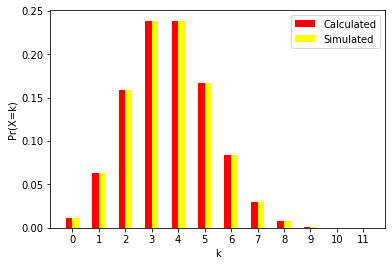
\includegraphics[width=\columnwidth,scale=0.9]{Assignment-5.png}
\end{document}